% =====================================================================
%  neuralCSCG -- Research Presentation
%  Compile with:  pdflatex presentation.tex   (run twice)
%  Figures expected in ./figures/
%  Custom modern theme (no external theme dependency).
% =====================================================================
\documentclass[aspectratio=169,10pt]{beamer}

\usepackage[utf8]{inputenc}
\usepackage[T1]{fontenc}
\usepackage{lmodern}
\usepackage{amsmath,amssymb,amsthm,mathtools}
\usepackage{graphicx}
\usepackage{booktabs}
\usepackage{array}
\usepackage{xcolor}
\usepackage{tikz}
\usetikzlibrary{arrows.meta,positioning,calc,fit,backgrounds,shapes.geometric,decorations.pathreplacing}
\usepackage{microtype}
\usepackage{appendixnumberbeamer}

\graphicspath{{figures/}}

% ------- Math shortcuts -------
\DeclareMathOperator*{\lse}{logsumexp}
\DeclareMathOperator*{\argmax}{arg\,max}
\DeclareMathOperator*{\argmin}{arg\,min}
\newcommand{\sg}{\operatorname{sg}}
\newcommand{\R}{\mathbb{R}}
\newcommand{\Lcal}{\mathcal{L}}

% =====================================================================
%  Custom theme: deep navy + warm gold
% =====================================================================
\definecolor{deepblue}{HTML}{0B2447}
\definecolor{midblue}{HTML}{19376D}
\definecolor{accentgold}{HTML}{C9A86A}
\definecolor{softgray}{HTML}{EFEFE7}
\definecolor{textdark}{HTML}{2A2A2A}
\definecolor{mutedgray}{HTML}{777777}
\definecolor{goodgreen}{HTML}{2E8B57}
\definecolor{badred}{HTML}{B0413E}

\setbeamercolor{normal text}{fg=textdark,bg=white}
\setbeamercolor{structure}{fg=deepblue}
\setbeamercolor{frametitle}{fg=deepblue,bg=white}
\setbeamercolor{title}{fg=deepblue}
\setbeamercolor{subtitle}{fg=mutedgray}
\setbeamercolor{author}{fg=textdark}
\setbeamercolor{date}{fg=mutedgray}
\setbeamercolor{section in toc}{fg=deepblue}
\setbeamercolor{itemize item}{fg=accentgold}
\setbeamercolor{itemize subitem}{fg=accentgold}
\setbeamercolor{itemize subsubitem}{fg=accentgold}
\setbeamercolor{enumerate item}{fg=deepblue}
\setbeamercolor{block title}{fg=white,bg=deepblue}
\setbeamercolor{block body}{fg=textdark,bg=softgray}
\setbeamercolor{alerted text}{fg=accentgold}

\setbeamerfont{frametitle}{size=\Large,series=\bfseries}
\setbeamerfont{title}{size=\huge,series=\bfseries}
\setbeamerfont{subtitle}{size=\normalsize,shape=\itshape}
\setbeamerfont{author}{size=\normalsize}
\setbeamerfont{block title}{series=\bfseries}

\setbeamertemplate{navigation symbols}{}
\setbeamertemplate{itemize item}{\raisebox{0.3ex}{\scriptsize$\blacksquare$}}
\setbeamertemplate{itemize subitem}{\raisebox{0.4ex}{\tiny$\square$}}

% --- Frame title: bold navy, thin gold underline
\setbeamertemplate{frametitle}{%
  \nointerlineskip
  \vspace*{0.7em}%
  \begin{beamercolorbox}[wd=\paperwidth,leftskip=1.2em,rightskip=1.2em]{frametitle}%
    \insertframetitle\par
    \vspace*{0.15em}%
    {\color{accentgold}\rule{\dimexpr\paperwidth-2.4em\relax}{1.0pt}}%
  \end{beamercolorbox}%
  \vspace*{0.4em}%
}

% --- Footer: tiny, author left, title + page right
\setbeamertemplate{footline}{%
  \leavevmode%
  \hbox{%
    \begin{beamercolorbox}[wd=0.5\paperwidth,ht=2.4ex,dp=1ex,leftskip=1.2em]{author}%
      \tiny\color{mutedgray}\insertshortauthor%
    \end{beamercolorbox}%
    \begin{beamercolorbox}[wd=0.5\paperwidth,ht=2.4ex,dp=1ex,rightskip=1.2em]{date}%
      \tiny\color{mutedgray}\hfill\insertshorttitle\quad\textbf{\insertframenumber}/\inserttotalframenumber%
    \end{beamercolorbox}%
  }\vskip0pt%
}

% --- Section divider slides: deep blue full background
\AtBeginSection[]{
  \begin{frame}[plain,noframenumbering]
    \begin{tikzpicture}[remember picture,overlay]
      \fill[deepblue] (current page.south west) rectangle (current page.north east);
      \node[anchor=west,xshift=1.6cm,yshift=0.6cm] at (current page.west) {%
        \begin{minipage}{0.9\paperwidth}
          {\color{accentgold}\rule{1.6em}{2.5pt}}\\[1.0em]
          {\color{white}\fontsize{14}{16}\selectfont\textsc{Part \thesection}}\\[0.7em]
          {\color{white}\fontsize{30}{34}\selectfont\bfseries\insertsection}
        \end{minipage}
      };
    \end{tikzpicture}
  \end{frame}
}

% --- Custom block style
\setbeamertemplate{blocks}[rounded][shadow=false]

% =====================================================================
%  Title
% =====================================================================
\title[neuralCSCG]{From Cognitive Maps to Neural Architectures}
\subtitle{A Gradient-Based, End-to-End Differentiable CSCG Pipeline}
\author[A. Nikzad]{Arash Nikzad \\[0.3em] {\small Supervisor: Dr.~Tristan Stober}}
\institute{}
\date{\today}

\begin{document}

% =====================================================================
%  Title slide
% =====================================================================
\begin{frame}[plain,noframenumbering]
  
\begin{tikzpicture}[remember picture,overlay]
    % Top accent band
    \fill[deepblue] (current page.north west) rectangle ([yshift=-2.9cm]current page.north east);
    \fill[accentgold] ([yshift=-2.9cm]current page.north west) rectangle ([yshift=-3.05cm]current page.north east);

    % Bottom accent band
    \fill[deepblue!8] ([yshift=2.2cm]current page.south west) rectangle (current page.south east);
    \fill[accentgold] ([yshift=2.35cm]current page.south west) rectangle ([yshift=2.2cm]current page.south east);

    % Title block over top band
    \node[anchor=west,xshift=1.2cm,yshift=-1.3cm] at (current page.north west) {%
      \begin{minipage}{0.9\paperwidth}
        \raggedright
        {\color{white}\fontsize{24}{28}\selectfont\bfseries From Cognitive Maps\\ to Neural Architectures}\\[0.5em]
        {\color{accentgold}\fontsize{13}{16}\selectfont\itshape A Gradient-Based, End-to-End Differentiable CSCG Pipeline}
      \end{minipage}
    };

    % Author block in middle
    \node[anchor=center] at ([yshift=-0.6cm]current page.center) {%
      \begin{minipage}{0.8\paperwidth}
        \centering
        {\color{deepblue}\fontsize{18}{22}\selectfont\bfseries Arash Nikzad}\\[0.4em]
        {\color{mutedgray}\fontsize{12}{14}\selectfont\itshape Supervisor: Dr.~Tristan Stober}\\[1.2em]
        {\color{accentgold}\rule{2em}{1.2pt}}
      \end{minipage}
    };

    % Date and project at bottom band
    \node[anchor=south,yshift=0.9cm] at (current page.south) {%
      \color{deepblue}\small\textsc{neuralCSCG} \quad$\cdot$\quad Research Presentation \quad$\cdot$\quad \today%
    };
  \end{tikzpicture}
\end{frame}

% =====================================================================
%  Roadmap
% =====================================================================
\begin{frame}{Roadmap}
  \vspace{0.4em}
  \begin{columns}[T,onlytextwidth]
    \begin{column}{0.5\textwidth}
      \begin{enumerate}\setlength\itemsep{0.55em}
        \item[\textbf{I.}] \textbf{Why CSCGs?} \\
              \small\color{mutedgray}Cognitive maps and the hippocampal connection
        \item[\textbf{II.}] \textbf{Gradient-Based CSCG}\\
              \small\color{mutedgray}From EM to differentiable forward in log-space
        \item[\textbf{III.}] \textbf{Adding Vision (VQ-VAE)}\\
              \small\color{mutedgray}A soft-emission bridge to perception
      \end{enumerate}
    \end{column}
    \begin{column}{0.5\textwidth}
      \begin{enumerate}\setlength\itemsep{0.55em}
        \item[\textbf{IV.}] \textbf{Joint Training}\\
              \small\color{mutedgray}Phased schedule, loss balancing, stability
        \item[\textbf{V.}] \textbf{Experiments}\\
              \small\color{mutedgray}MNIST gridworld and topology recovery
        \item[\textbf{VI.}] \textbf{What's Next}\\
              \small\color{mutedgray}Dynamic clones, RNN-CSCG, exponential state machines
      \end{enumerate}
    \end{column}
  \end{columns}
\end{frame}

% =====================================================================
\section{Why CSCGs?}
% =====================================================================

\begin{frame}{Cognitive maps from streams of experience}
  \begin{columns}[T,onlytextwidth]
    \begin{column}{0.52\textwidth}
      \begin{itemize}\setlength\itemsep{0.5em}
        \item An agent receives $(o_t, a_t)$ from interaction with the world.
        \item It must infer a \textbf{structured internal model} of the
              environment --- a \emph{cognitive map}.
        \item \textbf{Clone-Structured Cognitive Graphs (CSCGs)} are an
              action-augmented \emph{cloned HMM} that have been shown to
              recover environment topology under perceptual aliasing.
        \item Each observation symbol owns several latent \emph{clones};
              context disambiguates aliased percepts.
      \end{itemize}
    \end{column}
    \begin{column}{0.48\textwidth}
      \centering
      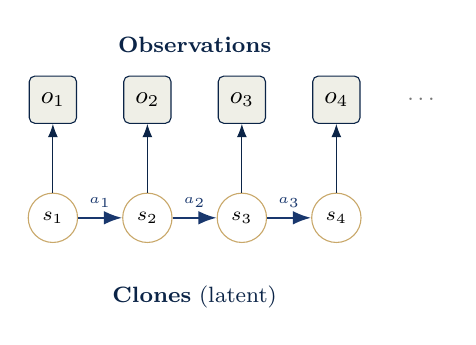
\begin{tikzpicture}[
        >=Latex,
        obs/.style={draw=deepblue,fill=softgray,rounded corners=2pt,
                    minimum size=6mm,font=\small\bfseries},
        clone/.style={draw=accentgold,fill=white,circle,
                      minimum size=5mm,font=\scriptsize},
        every node/.style={align=center}
      ]
        \node[obs] (o1) at (0,3) {$o_1$};
        \node[obs] (o2) at (1.2,3) {$o_2$};
        \node[obs] (o3) at (2.4,3) {$o_3$};
        \node[obs] (o4) at (3.6,3) {$o_4$};
        \node[font=\footnotesize,mutedgray] at (4.7,3) {\dots};

        \node[clone] (s1) at (0,1.5) {$s_1$};
        \node[clone] (s2) at (1.2,1.5) {$s_2$};
        \node[clone] (s3) at (2.4,1.5) {$s_3$};
        \node[clone] (s4) at (3.6,1.5) {$s_4$};

        \draw[->,deepblue] (s1)--(o1);
        \draw[->,deepblue] (s2)--(o2);
        \draw[->,deepblue] (s3)--(o3);
        \draw[->,deepblue] (s4)--(o4);

        \draw[->,midblue,thick] (s1)--node[above,font=\tiny]{$a_1$}(s2);
        \draw[->,midblue,thick] (s2)--node[above,font=\tiny]{$a_2$}(s3);
        \draw[->,midblue,thick] (s3)--node[above,font=\tiny]{$a_3$}(s4);

        \node[font=\footnotesize,deepblue] at (1.8,0.5){\textbf{Clones} (latent)};
        \node[font=\footnotesize,deepblue] at (1.8,3.7){\textbf{Observations}};
      \end{tikzpicture}
    \end{column}
  \end{columns}
\end{frame}

\begin{frame}{Why focus on CSCGs in particular?}
  \begin{block}{A neuroscientific anchor}
    \textit{``Learning produces an orthogonalized state machine in the
    hippocampus''} (Sun et al., 2023; \emph{Nature}) showed that the
    \textbf{activations of a CSCG model are the closest match to
    hippocampal recordings}, among the model classes tested.
  \end{block}
  \vspace{0.4em}
  \begin{itemize}\setlength\itemsep{0.4em}
    \item This suggests CSCGs carry a \textbf{useful inductive bias} for
          building cognitive maps.
    \item If the bias is biologically aligned, it is worth scaling --- but
          today's CSCGs are not built for scale.
    \item \textbf{Working hypothesis:} make the inductive bias of CSCGs
          \emph{trainable inside modern neural pipelines}.
  \end{itemize}
\end{frame}

\begin{frame}{The limitation: CSCGs sit on an old foundation}
  \begin{columns}[T,onlytextwidth]
    \begin{column}{0.55\textwidth}
      \begin{itemize}\setlength\itemsep{0.45em}
        \item CSCGs are an \textbf{HMM} --- a probabilistic model from the 1960s.
        \item Trained with \textbf{Expectation-Maximization} (Baum--Welch):
        \begin{itemize}
          \item \textbf{E-step:} forward--backward to get posteriors.
          \item \textbf{M-step:} closed-form re-estimation of $\pi, T, B$.
        \end{itemize}
        \item Closed-form M-step requires \emph{conjugate} emission structure.
        \item No mechanism to \textbf{compose} a CSCG with a CNN, a VQ-VAE,
              or any other neural module.
        \item Discrete observation alphabet must be supplied \emph{from
              outside}.
      \end{itemize}
    \end{column}
    \begin{column}{0.42\textwidth}
      \centering
      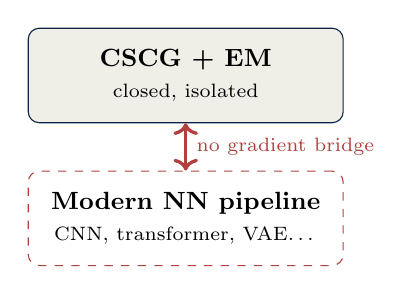
\begin{tikzpicture}[font=\small]
        \node[draw=deepblue,fill=softgray,rounded corners,
              minimum width=4cm,minimum height=1.2cm,align=center] (em) {%
              \textbf{CSCG + EM}\\\scriptsize closed, isolated};
        \node[draw=badred,dashed,rounded corners,
              minimum width=4cm,minimum height=1.2cm,align=center,
              below=0.6cm of em] (nn) {%
              \textbf{Modern NN pipeline}\\\scriptsize CNN, transformer, VAE\dots};
        \draw[<->,badred,very thick] (em) -- node[right,font=\scriptsize]{no gradient bridge} (nn);
      \end{tikzpicture}
    \end{column}
  \end{columns}
\end{frame}

% =====================================================================
\section{Gradient-Based CSCG}
% =====================================================================

\begin{frame}{Step 1 --- a gradient-trained CSCG}
  \begin{block}{Goal}
    Replace EM with stochastic gradient descent so the CSCG becomes a
    \textbf{drop-in differentiable module}.
  \end{block}
  \vspace{0.4em}
  \begin{itemize}\setlength\itemsep{0.45em}
    \item Express the forward algorithm as a \textbf{log-space computational
          graph}.
    \item Optimize the negative log-likelihood directly with Adam.
    \item Use \texttt{logsumexp} for numerical stability over long episodes.
    \item Result: an action-conditioned CSCG that is end-to-end
          \textbf{differentiable in its parameters} $(\pi, \Theta)$.
  \end{itemize}
  \vspace{0.4em}
  \begin{center}
    \color{deepblue}\itshape
    This is the prerequisite for everything that follows --- once trainable
    by gradients, the CSCG can sit inside any neural pipeline.
  \end{center}
\end{frame}

\begin{frame}{Math --- the classical HMM forward}
  \textbf{Setup.}\; Hidden states $s_t \in \mathcal{S}=\{1,\dots,N\}$,
  observations $o_t \in \{1,\dots,K\}$, actions $a_t \in \{1,\dots,A\}$.
  \begin{itemize}
    \item Initial distribution: $\bar\pi_j = \mathrm{softmax}(\pi)_j$.
    \item Transitions: $T_{a,i,j} = \mathrm{softmax}_j(\Theta_{a,i,\cdot})$.
    \item Emissions (CSCG): \textbf{deterministic}, $B_{s,o}=\mathbb{1}[\omega(s)=o]$.
  \end{itemize}

  \vspace{0.3em}
  \textbf{Forward recursion} ($\alpha_t(j) = P(o_{1:t}, s_t = j \mid a_{1:t-1})$):
  \begin{align*}
    \alpha_1(j) &= \bar\pi_j\, B_{j,o_1}\\
    \alpha_{t+1}(j) &= \Bigl[\textstyle\sum_i \alpha_t(i)\, T_{a_t,i,j}\Bigr]\, B_{j,o_{t+1}}
  \end{align*}

  \vspace{0.2em}
  \textbf{Likelihood:}\quad
  $P(o_{1:T} \mid a_{1:T-1}) = \sum_j \alpha_T(j)$.

  \vspace{0.6em}
  \begin{block}{Two problems with raw $\alpha$'s}
    \begin{enumerate}
      \item \textbf{Numerical underflow} on long $T$.
      \item Classical EM re-estimates parameters in closed form ---
            \emph{not} via gradients.
    \end{enumerate}
  \end{block}
\end{frame}

\begin{frame}{From EM to gradient descent: the log-space forward}
  \textbf{Idea.}\; Work in log-space, replace sums by $\lse$, treat the whole
  recursion as a TensorFlow graph; gradients flow into $(\pi,\Theta)$ via
  backprop.

  \vspace{0.2em}
  Let $\lse_i u_i \;=\; \log \sum_i e^{u_i}$. The log-forward messages are
  \begin{align*}
    \log\alpha_1(j) &= \log\bar\pi_j + \log B_{j,o_1},\\[-1pt]
    \log\alpha_{t+1}(j) &= \lse_i\bigl[\log\alpha_t(i) + \log T_{a_t,i,j}\bigr] + \log B_{j,o_{t+1}}.
  \end{align*}

  \vspace{-0.4em}
  Episode log-likelihood and NLL:\;
  $\displaystyle\ell = \lse_j \log\alpha_T(j),\quad
   \Lcal_{\text{HMM}} = -\tfrac{1}{|\mathcal{B}|}\!\sum \ell$.

  \vspace{0.3em}
  \begin{columns}[T,onlytextwidth]
    \begin{column}{0.46\textwidth}
      \textbf{Parameter update (gradient):}
      \[
        (\pi,\Theta) \;\leftarrow\; (\pi,\Theta) - \eta\,\nabla \Lcal_{\text{HMM}}.
      \]
    \end{column}
    \begin{column}{0.54\textwidth}
      \textbf{Why this is enough:}
      \begin{itemize}\small
        \item Softmax keeps $\bar\pi, T$ normalized.
        \item $\lse$ is smooth, exact, stable.
        \item No conjugacy assumption; composable with any upstream module.
      \end{itemize}
    \end{column}
  \end{columns}
\end{frame}

\begin{frame}{gradCSCG --- summary of the first step}
  \begin{columns}[T,onlytextwidth]
    \begin{column}{0.58\textwidth}
      \begin{itemize}\small\setlength\itemsep{0.4em}
        \item Same model class as the classical CSCG, same clone semantics.
        \item Trained by SGD/Adam on the log-space forward NLL.
        \item Masked, batched recursion over padded minibatches.
        \item Viterbi decoding stays available for evaluation.
      \end{itemize}
      \vspace{0.4em}
      \begin{block}{Why it matters}
        gradCSCG is the \emph{interface} between the cognitive-map
        inductive bias and the rest of deep learning.
      \end{block}
    \end{column}
    \begin{column}{0.42\textwidth}
      \centering
      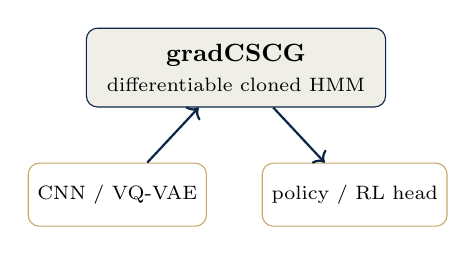
\begin{tikzpicture}[font=\small]
        \node[draw=deepblue,fill=softgray,rounded corners,
              minimum width=3.8cm,minimum height=1.0cm,align=center] (g)
              {\textbf{gradCSCG}\\\scriptsize differentiable cloned HMM};
        \node[draw=accentgold,rounded corners,minimum width=1.9cm,
              minimum height=0.8cm,below=0.7cm of g.south west,
              anchor=north,align=center,xshift=0.4cm]
              (cnn) {\scriptsize CNN / VQ-VAE};
        \node[draw=accentgold,rounded corners,minimum width=1.9cm,
              minimum height=0.8cm,below=0.7cm of g.south east,
              anchor=north,align=center,xshift=-0.4cm]
              (rl)  {\scriptsize policy / RL head};
        \draw[->,deepblue,thick] (cnn) -- (g);
        \draw[->,deepblue,thick] (g) -- (rl);
      \end{tikzpicture}
    \end{column}
  \end{columns}
\end{frame}

% =====================================================================
\section{Adding Vision via VQ-VAE}
% =====================================================================

\begin{frame}{From integer observations to images}
  \begin{columns}[T,onlytextwidth]
    \begin{column}{0.5\textwidth}
      \textbf{Today's CSCG observation:}
      \begin{itemize}
        \item a single integer $o_t \in \{1,\dots,K\}$.
        \item Assumes someone else has discretized the world for us.
      \end{itemize}
      \vspace{0.4em}
      \textbf{What a real agent sees:}
      \begin{itemize}
        \item pixels --- high-dimensional, noisy, aliased.
        \item the same place can look different each visit.
      \end{itemize}
      \vspace{0.5em}
      \begin{block}{Plan}
        Give the CSCG \textbf{eyes}: a \emph{VQ-VAE} maps each image to a
        learned discrete token; gradCSCG consumes those tokens.
      \end{block}
    \end{column}
    \begin{column}{0.5\textwidth}
      \centering
      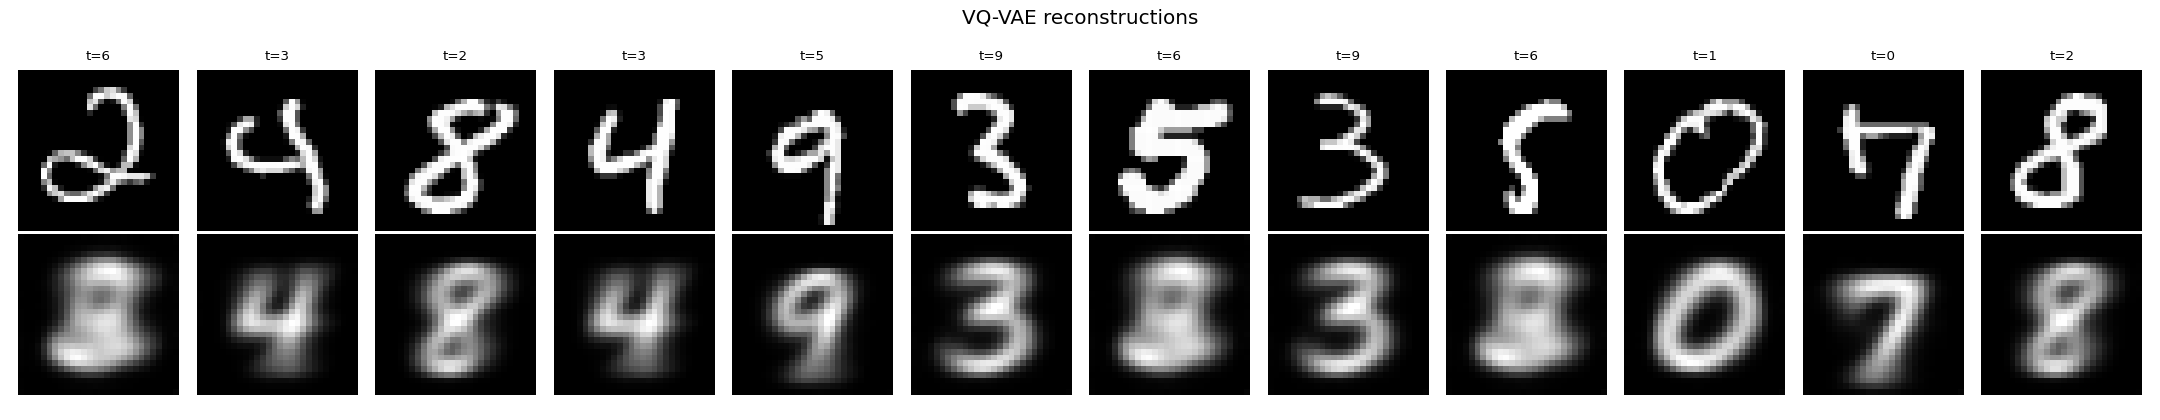
\includegraphics[width=0.92\linewidth]{reconstructions.png}\\
      {\scriptsize\color{mutedgray}Top: input images.\;
       Bottom: VQ-VAE reconstructions and assigned token id.}
    \end{column}
  \end{columns}
\end{frame}

\begin{frame}{The neuralCSCG pipeline}
  \centering
  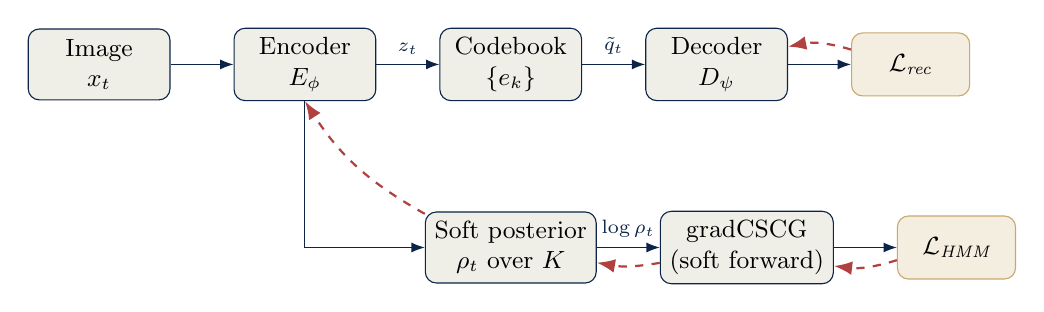
\begin{tikzpicture}[
    >=Latex, node distance=6mm and 8mm,
    box/.style={draw=deepblue,fill=softgray,rounded corners,
                minimum height=9mm,minimum width=18mm,align=center,
                font=\small},
    loss/.style={draw=accentgold,fill=accentgold!20,rounded corners,
                 minimum height=8mm,minimum width=15mm,align=center,
                 font=\small\itshape},
    grad/.style={->,dashed,badred,thick}
  ]
    \node[box] (img)  {Image\\$x_t$};
    \node[box, right=of img] (enc)  {Encoder\\$E_\phi$};
    \node[box, right=of enc] (vq)   {Codebook\\$\{e_k\}$};
    \node[box, right=of vq]  (dec)  {Decoder\\$D_\psi$};
    \node[loss, right=of dec] (rec) {$\Lcal_{\text{rec}}$};

    \node[box, below=14mm of vq] (soft) {Soft posterior\\$\rho_t$ over $K$};
    \node[box, right=of soft] (hmm) {gradCSCG\\(soft forward)};
    \node[loss, right=of hmm] (nll) {$\Lcal_{\text{HMM}}$};

    \draw[->,deepblue] (img)--(enc);
    \draw[->,deepblue] (enc)--node[above,font=\scriptsize]{$z_t$}(vq);
    \draw[->,deepblue] (vq)--node[above,font=\scriptsize]{$\tilde q_t$}(dec);
    \draw[->,deepblue] (dec)--(rec);
    \draw[->,deepblue] (enc.south) |- (soft);
    \draw[->,deepblue] (soft)--node[above,font=\scriptsize]{$\log\rho_t$}(hmm);
    \draw[->,deepblue] (hmm)--(nll);

    \draw[grad] (rec) to[bend right=14] (dec);
    \draw[grad] (nll) to[bend left=12] (hmm);
    \draw[grad] (hmm) to[bend left=10] (soft);
    \draw[grad] (soft) to[bend left=14] (enc.south);
  \end{tikzpicture}
  \vspace{0.5em}\\[-0.2em]
  {\footnotesize\color{mutedgray}Solid: forward pass.\;
   Dashed red: gradient flow.\;
   Codebook updated by \textbf{EMA}, not by gradients.}
\end{frame}

\begin{frame}{The eye --- VQ-VAE: quantization \& straight-through}
  \textbf{Encoder + quantizer.}\; Convnet $E_\phi: x \mapsto z \in \R^{D}$;
  codebook $\{e_k\}_{k=1}^{K}\subset\R^{D}$.
  \[
    k_t = \argmin_k \|z_t - e_k\|_2^2, \qquad q_t = e_{k_t}.
  \]
  Gradients cross the non-differentiable $\argmin$ by the \textbf{straight-through estimator}:
  \[
    \tilde q_t = z_t + \sg(q_t - z_t),
    \qquad
    \frac{\partial \tilde q_t}{\partial z_t} = I.
  \]

  \textbf{Losses.}\quad
  $\Lcal_{\text{rec}} = \tfrac{1}{|\mathcal{B}|}\sum_t \|x_t - \hat x_t\|_2^2$,
  \quad
  $\Lcal_{\text{commit}} = \tfrac{1}{|\mathcal{B}|}\sum_t \|\sg(q_t) - z_t\|_2^2$.

  \vspace{0.4em}
  \textbf{Codebook (no gradient).}\; EMA updates per code $k$ with decay $\gamma$:
  \[
    n_k \leftarrow \gamma n_k + (1-\gamma)\!\sum_t \mathbb{1}[k_t=k],\quad
    m_k \leftarrow \gamma m_k + (1-\gamma)\!\sum_t \mathbb{1}[k_t=k]\,z_t,\quad
    e_k \leftarrow m_k / \hat n_k.
  \]
\end{frame}

\begin{frame}{The bridge --- soft codebook posterior}
  We need the HMM likelihood to be \textbf{differentiable in $z_t$} so that
  gradients reach the encoder. A hard $\argmin$ is not.

  \vspace{0.3em}
  \begin{block}{Temperature-controlled soft posterior over the codebook}
    \[
      \log \rho_t(k) \;=\; \log\mathrm{softmax}_k\!\Bigl(-\|z_t - e_k\|_2^2 \,/\, \tau\Bigr).
    \]
  \end{block}

  \vspace{0.3em}
  \textbf{Two key properties:}
  \begin{itemize}\setlength\itemsep{0.35em}
    \item \textbf{Differentiable in $z_t$} (so also in $\phi$).
    \item \textbf{Consistency:} as $\tau\to 0$, $\rho_t$ concentrates on
          $k_t$ and reduces to the hard one-hot assignment.
  \end{itemize}

  \vspace{0.4em}
  \begin{center}\itshape\color{deepblue}
    $\rho_t$ is the soft handshake between perception and sequence learning.
  \end{center}
\end{frame}

\begin{frame}{Soft-emission forward pass --- the key derivation}
  Recall: state $j$ deterministically emits token $\omega(j)$.
  In the hard forward, the emission term is $\log B_{j, o_t}$
  (i.e.\ $-\infty$ unless $\omega(j) = o_t$).

  \vspace{0.3em}
  \textbf{Replace the hard emission with the soft log-posterior of $\omega(j)$:}
  \begin{align*}
    \log\alpha^{s}_1(j) &= \log\bar\pi_j + \log\rho_1\!\bigl(\omega(j)\bigr) \\
    \log\alpha^{s}_{t+1}(j) &= \lse_i\bigl[\log\alpha^{s}_t(i) + \log T_{a_t,i,j}\bigr]
                                 + \log\rho_{t+1}\!\bigl(\omega(j)\bigr)
  \end{align*}

  \vspace{-0.4em}
  \textbf{Soft log-likelihood:}\quad
  $\ell^{s} = \lse_j \log\alpha^{s}_T(j)$.

  \vspace{0.5em}
  \begin{columns}[T,onlytextwidth]
    \begin{column}{0.5\textwidth}
      \textbf{Consistency (proof sketch).}\\
      If $\rho_t = \mathrm{onehot}(o_t)$, then
      $\log\rho_t(\omega(j))=\log B_{j,o_t}$, so the soft forward reduces
      \emph{exactly} to the hard forward as $\tau\to 0$.
    \end{column}
    \begin{column}{0.5\textwidth}
      \textbf{Why it matters.}\\
      Gradients propagate
      $\ell^{s}\to\rho\to z\to\phi$:
      the topological objective now \emph{shapes perception}.
    \end{column}
  \end{columns}
\end{frame}

% =====================================================================
\section{Joint Training}
% =====================================================================

\begin{frame}{The joint objective}
  \begin{block}{Combined loss at joint training step $t$}
    \[
      \Lcal_{\text{joint}} \;=\;
      \Lcal_{\text{rec}}
      \;+\; \beta\,\Lcal_{\text{commit}}
      \;+\; \lambda_t\, \widetilde{\Lcal}_{\text{HMM}}
      \;+\; \alpha_{\text{div}}\,\Lcal_{\text{div}}
    \]
  \end{block}

  \vspace{0.3em}
  \begin{itemize}\setlength\itemsep{0.35em}
    \item $\Lcal_{\text{rec}}, \Lcal_{\text{commit}}$ --- the VQ-VAE terms (perception stays faithful).
    \item $\widetilde{\Lcal}_{\text{HMM}}$ --- the \emph{length-normalized} soft NLL (topology pressure).
    \item $\Lcal_{\text{div}}$ --- diversity penalty (anti-collapse).
    \item $\lambda_t$ --- annealed sequence-loss weight.
  \end{itemize}

  \vspace{0.4em}
  \begin{center}\color{deepblue}\itshape
    Naive joint training collapses --- the next slide is why, and how we fix it.
  \end{center}
\end{frame}

\begin{frame}{Loss balancing --- the four knobs}
  \begin{columns}[T,onlytextwidth]
    \begin{column}{0.5\textwidth}
      \textbf{1. Length normalization}\\
      The raw NLL grows $O(T)$, dwarfing the $O(1)$ reconstruction term.
      \[
        \widetilde{\Lcal}_{\text{HMM}} = -\tfrac{1}{|\mathcal{B}|}\!\sum \tfrac{1}{T}\,\ell^{s}.
      \]

      \vspace{0.5em}
      \textbf{2. Weight annealing}\\
      Let the codebook stabilize under reconstruction before topology
      pressure switches on.
      \[
        \lambda_t = \lambda \cdot \min\!\Bigl(1,\; t/T_{\text{anneal}}\Bigr).
      \]
    \end{column}
    \begin{column}{0.5\textwidth}
      \textbf{3. Diversity penalty}\\
      Let $\bar\rho(k) = \tfrac{1}{|\mathcal{B}|}\sum_t \rho_t(k)$.
      \[
        \Lcal_{\text{div}} = \log K - H(\bar\rho) \;\ge\; 0.
      \]
      Vanishes only at uniform usage --- counters codebook collapse.

      \vspace{0.5em}
      \textbf{4. Anti-collapse safeguards}\\
      \begin{itemize}\setlength\itemsep{0.15em}
        \item Perplexity-monitored best-checkpoint snapshot.
        \item Optional $\lambda$-throttling and rollback.
        \item Dead-code revival from encoder cluster centroids.
      \end{itemize}
    \end{column}
  \end{columns}
\end{frame}

\begin{frame}{Three-phase training schedule}
  \centering
  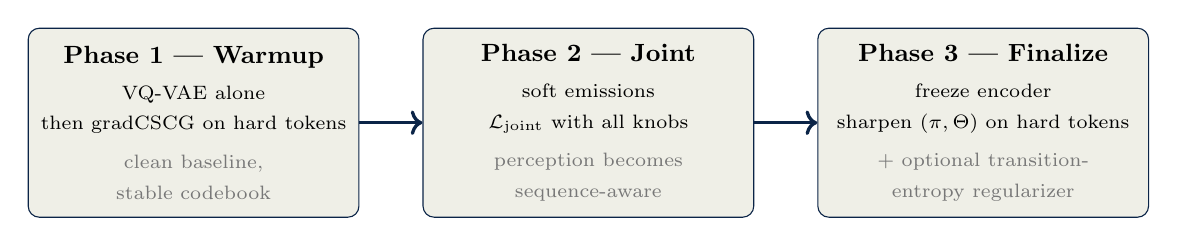
\begin{tikzpicture}[
    every node/.style={font=\small},
    phase/.style={draw=deepblue,fill=softgray,rounded corners,
                  minimum width=4.2cm,minimum height=2.4cm,align=center},
    arrow/.style={->,very thick,deepblue}
  ]
    \node[phase] (p1) {%
      \textbf{Phase 1 --- Warmup}\\[2pt]
      \scriptsize VQ-VAE alone\\
      \scriptsize then gradCSCG on hard tokens\\[3pt]
      \scriptsize\color{mutedgray}clean baseline,\\\scriptsize\color{mutedgray}stable codebook};
    \node[phase, right=0.8cm of p1] (p2) {%
      \textbf{Phase 2 --- Joint}\\[2pt]
      \scriptsize soft emissions\\
      \scriptsize $\Lcal_{\text{joint}}$ with all knobs\\[3pt]
      \scriptsize\color{mutedgray}perception becomes\\\scriptsize\color{mutedgray}sequence-aware};
    \node[phase, right=0.8cm of p2] (p3) {%
      \textbf{Phase 3 --- Finalize}\\[2pt]
      \scriptsize freeze encoder\\
      \scriptsize sharpen $(\pi,\Theta)$ on hard tokens\\[3pt]
      \scriptsize\color{mutedgray}+ optional transition-\\\scriptsize\color{mutedgray}entropy regularizer};
    \draw[arrow] (p1) -- (p2);
    \draw[arrow] (p2) -- (p3);
  \end{tikzpicture}

  \vspace{0.8em}
  \begin{itemize}\setlength\itemsep{0.1em}
    \item Phase 1 gives a strong baseline and prevents Phase 2 from starting in a bad basin.
    \item Phase 2 is where soft emissions actually couple the two modules.
    \item Phase 3 produces the final, sharp transition matrix used at evaluation.
  \end{itemize}
\end{frame}

\begin{frame}{One joint training step --- the algorithm}
  \begin{block}{Per-batch update}
  \begin{enumerate}\setlength\itemsep{0.15em}
    \item \textbf{Encode:} $z_t \gets E_\phi(x_t)$.
    \item \textbf{Quantize:} $q_t, \tilde q_t \gets$ quantize$(z_t)$; update codebook by EMA.
    \item \textbf{Reconstruct:} $\hat x_t \gets D_\psi(\tilde q_t)$;
          compute $\Lcal_{\text{rec}}, \Lcal_{\text{commit}}$.
    \item \textbf{Soft posterior:}
          $\log\rho_t \gets \log\mathrm{softmax}(-\|z_t - e_\cdot\|^2/\tau)$.
    \item \textbf{Soft forward:} run log-space recursion, get $\ell^{s}$.
    \item \textbf{Balance:}
          $\widetilde{\Lcal}_{\text{HMM}} \gets -\ell^{s}/T$;\;
          $\Lcal_{\text{div}} \gets \log K - H(\bar\rho)$.
    \item \textbf{Joint loss:}
          $\Lcal_{\text{joint}} = \Lcal_{\text{rec}} + \beta \Lcal_{\text{commit}} + \lambda_t \widetilde{\Lcal}_{\text{HMM}} + \alpha_{\text{div}} \Lcal_{\text{div}}$.
    \item \textbf{Update} $(\phi, \psi, \pi, \Theta)$ with Adam on $\nabla\Lcal_{\text{joint}}$.
  \end{enumerate}
  \end{block}
\end{frame}

% =====================================================================
\section{Experiments \& Results}
% =====================================================================

\begin{frame}{Does it work? --- the MNIST gridworld benchmark}
  \begin{columns}[T,onlytextwidth]
    \begin{column}{0.58\textwidth}
      \begin{itemize}\setlength\itemsep{0.35em}
        \item 2-D grid; each cell carries a \textbf{digit class}.
        \item \emph{Visiting a cell returns a random MNIST sample of that digit.}\\
              {\scriptsize\color{mutedgray}$\Rightarrow$ same place never looks identical twice.}
        \item Cells sharing a digit are \textbf{perceptually aliased}.
        \item Four actions (up/down/left/right) with sticky walls.
        \item Ground-truth topology is exactly known $\Rightarrow$ controlled
              testbed for \textbf{topology recovery}.
      \end{itemize}
    \end{column}
    \begin{column}{0.42\textwidth}
      \centering
      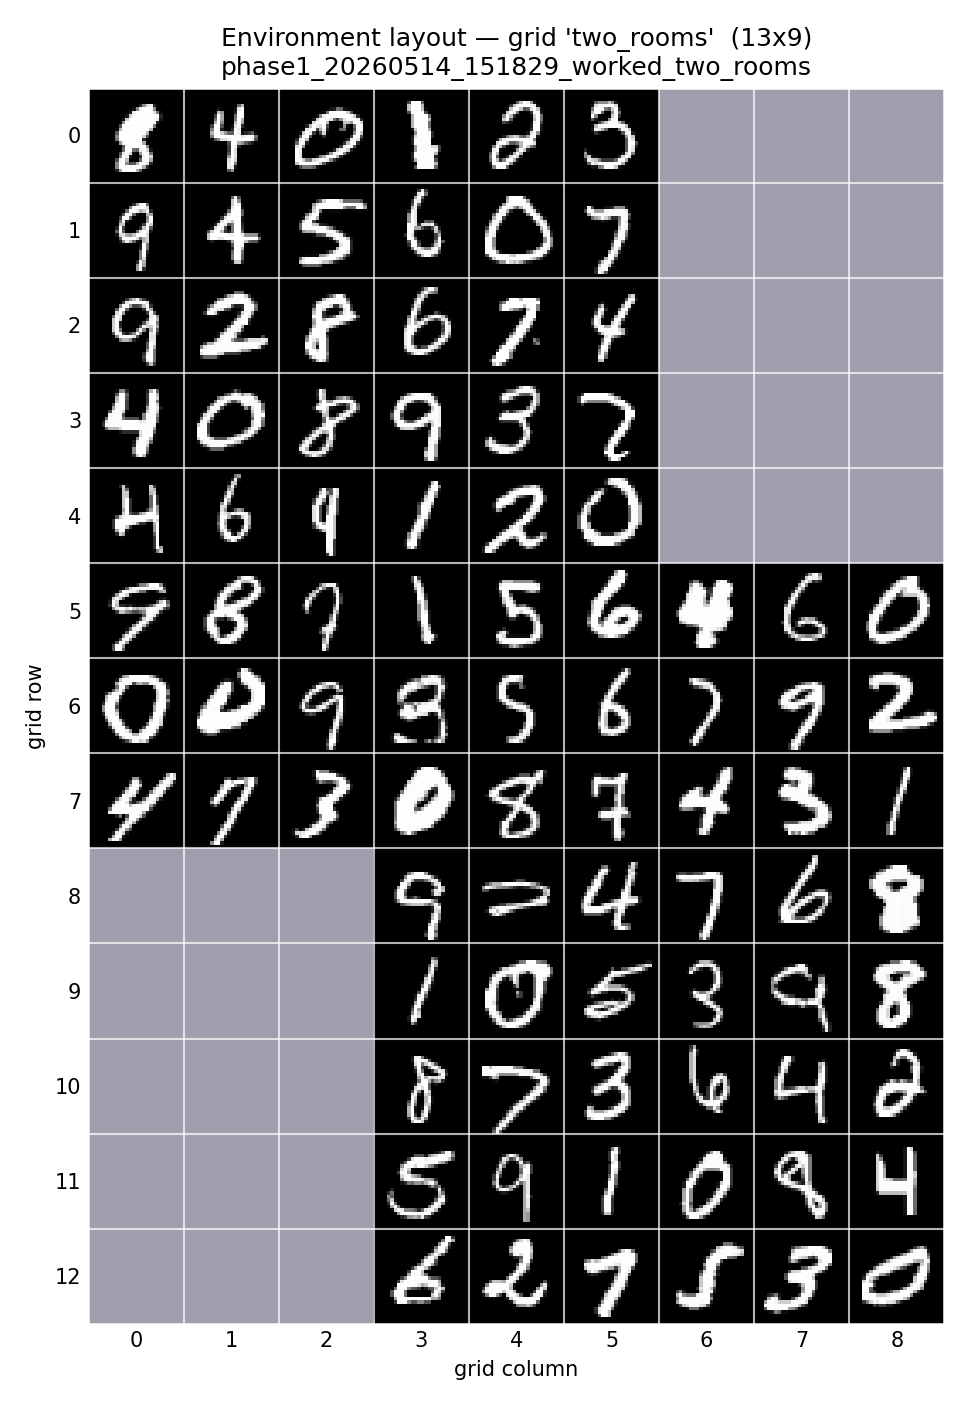
\includegraphics[height=0.62\textheight,keepaspectratio]{environment.png}\\[-0.1em]
      {\scriptsize\color{mutedgray}\texttt{two\_rooms} ($13\times 9$): two
       offset rooms; shared digits cause aliasing.}
    \end{column}
  \end{columns}
\end{frame}

\begin{frame}{Five benchmark environments}
  \centering
  \small
  \begin{tabular}{@{}lcccc@{}}
    \toprule
    \textbf{Environment} & \textbf{Grid} & \textbf{Tokens $K$} & \textbf{Clone states $N$} & \textbf{Character}\\
    \midrule
    \texttt{aliased}            & $4\times 4$   & $4$  & $21$  & 4 digits, each $\times 4$ --- controlled aliasing\\
    \texttt{corridors}          & $5\times 5$   & $6$  & $31$  & walls + repeats along corridors\\
    \texttt{room} (uniform)     & $6\times 6$   & $10$ & $201$ & rectangular room, uniform clones\\
    \texttt{room} (dynamic)     & $6\times 6$   & $10$ & $57$  & dynamic clone allocation\\
    \texttt{two\_rooms}         & $13\times 9$  & $10$ & $151$ & two interconnected rooms (hardest)\\
    \bottomrule
  \end{tabular}

  \vspace{0.8em}
  \begin{itemize}
    \item Trajectories: action-conditioned random walks --- $4$--$10$ episodes of $10{,}000$ steps.
    \item Optional coverage-biased rollout for rare $(\text{cell}, \text{action})$ pairs.
    \item All five environments run through the full Phase 2 $\to$ finalization pipeline.
  \end{itemize}
\end{frame}

\begin{frame}{Results I --- perception is clean}
  \begin{columns}[T,onlytextwidth]
    \begin{column}{0.5\textwidth}
      \centering
      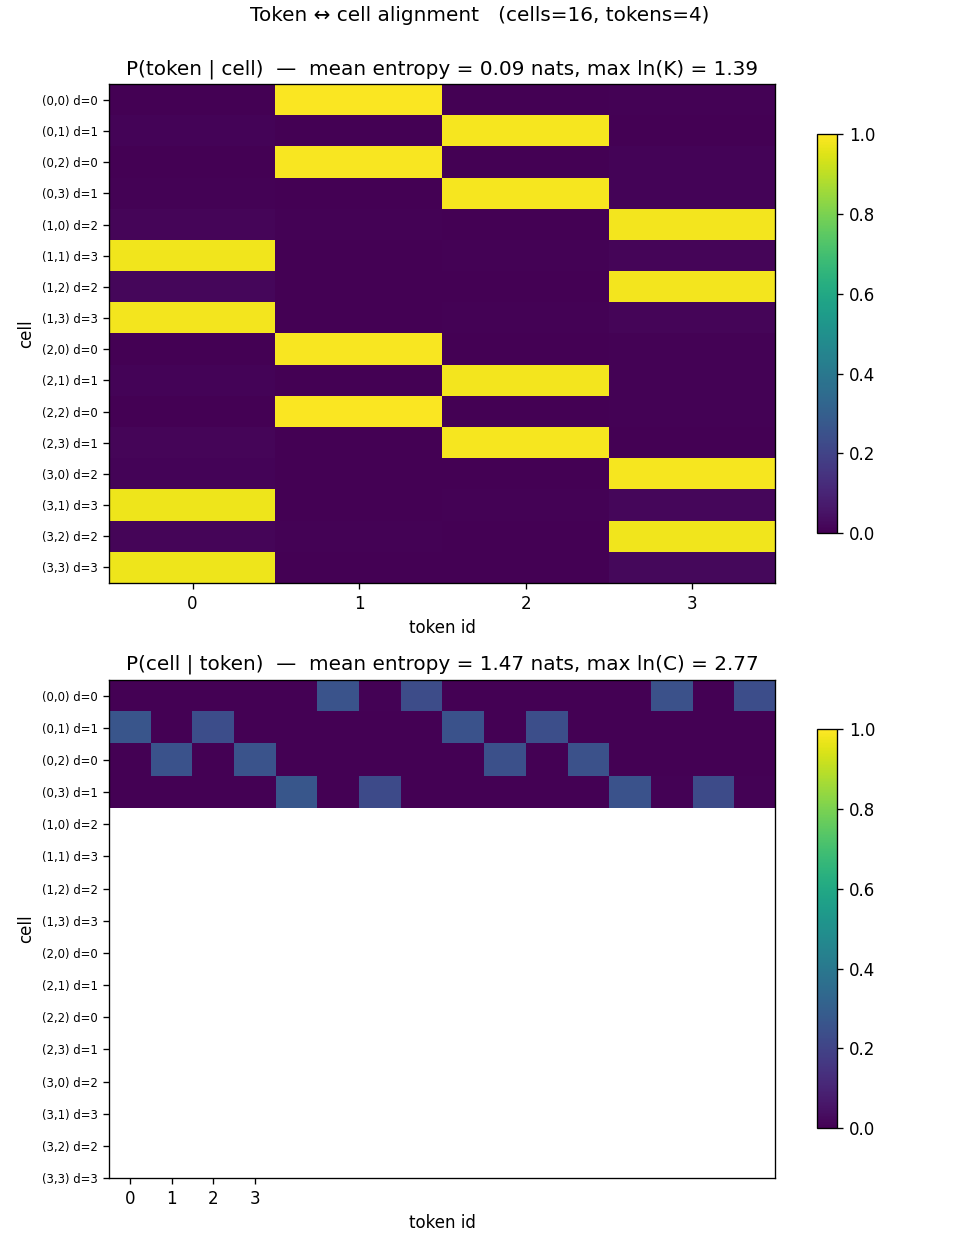
\includegraphics[height=0.62\textheight,keepaspectratio]{token_cell_heatmap.png}\\[-0.1em]
      {\scriptsize\color{mutedgray}Token$\leftrightarrow$place alignment (\texttt{aliased}).
       Top: $P(\text{token}\mid\text{place})$. Bottom: $P(\text{place}\mid\text{token})$.}
    \end{column}
    \begin{column}{0.5\textwidth}
      \centering
      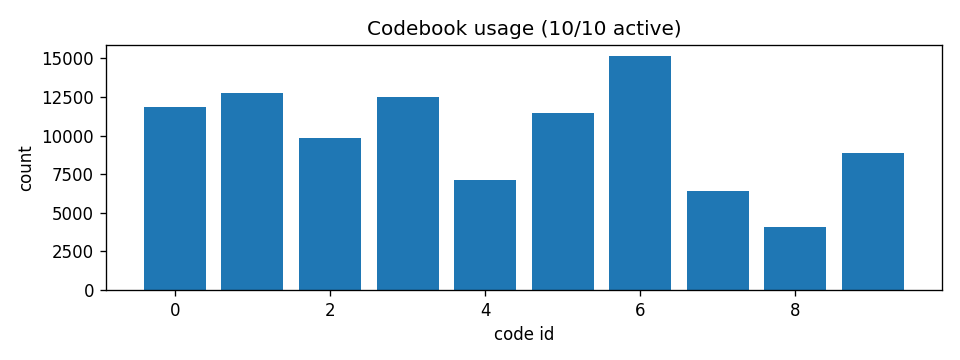
\includegraphics[width=0.92\linewidth]{codebook_usage.png}\\[-0.1em]
      {\scriptsize\color{mutedgray}Codebook utilization on \texttt{two\_rooms} --- all codes active.}
      \vspace{0.3em}
      \begin{itemize}\scriptsize\setlength\itemsep{0.15em}
        \item Mean tokens per cell: $\mathbf{1.0\text{--}1.2}$.
        \item $H(\text{token}\mid\text{place}) = 0.09\text{--}0.23$ nats.
        \item Perplexity $\approx$ number of digit classes; no collapse.
      \end{itemize}
    \end{column}
  \end{columns}
\end{frame}

\begin{frame}{Results II --- clones absorb the aliasing}
  \begin{columns}[T,onlytextwidth]
    \begin{column}{0.46\textwidth}
      \centering
      
\includegraphics[height=0.62\textheight,keepaspectratio]{viterbi_graph.png}\\[-0.1em]
      {\scriptsize\color{mutedgray}Decoded clone-state graph for \texttt{two\_rooms}: each node is an MNIST sample of the digit it represents.}
    \end{column}
    \begin{column}{0.52\textwidth}
      \begin{itemize}\small\setlength\itemsep{0.3em}
        \item Clones map cleanly to physical places.
        \item Visit-weighted \textbf{state-to-place purity = 0.95--0.98}.
        \item Every visited place is represented by at least one clone.
        \item Decoded clone graph already exposes the recovered topology.
      \end{itemize}
      \vspace{0.3em}
      \begin{block}{Take-away}
        The CSCG inductive bias survives the move to gradient training
        \emph{and} the move to learned visual tokens.
      \end{block}
    \end{column}
  \end{columns}
\end{frame}

\begin{frame}{Results III --- topology is recovered}
  \begin{columns}[T,onlytextwidth]
    \begin{column}{0.48\textwidth}
      \centering
      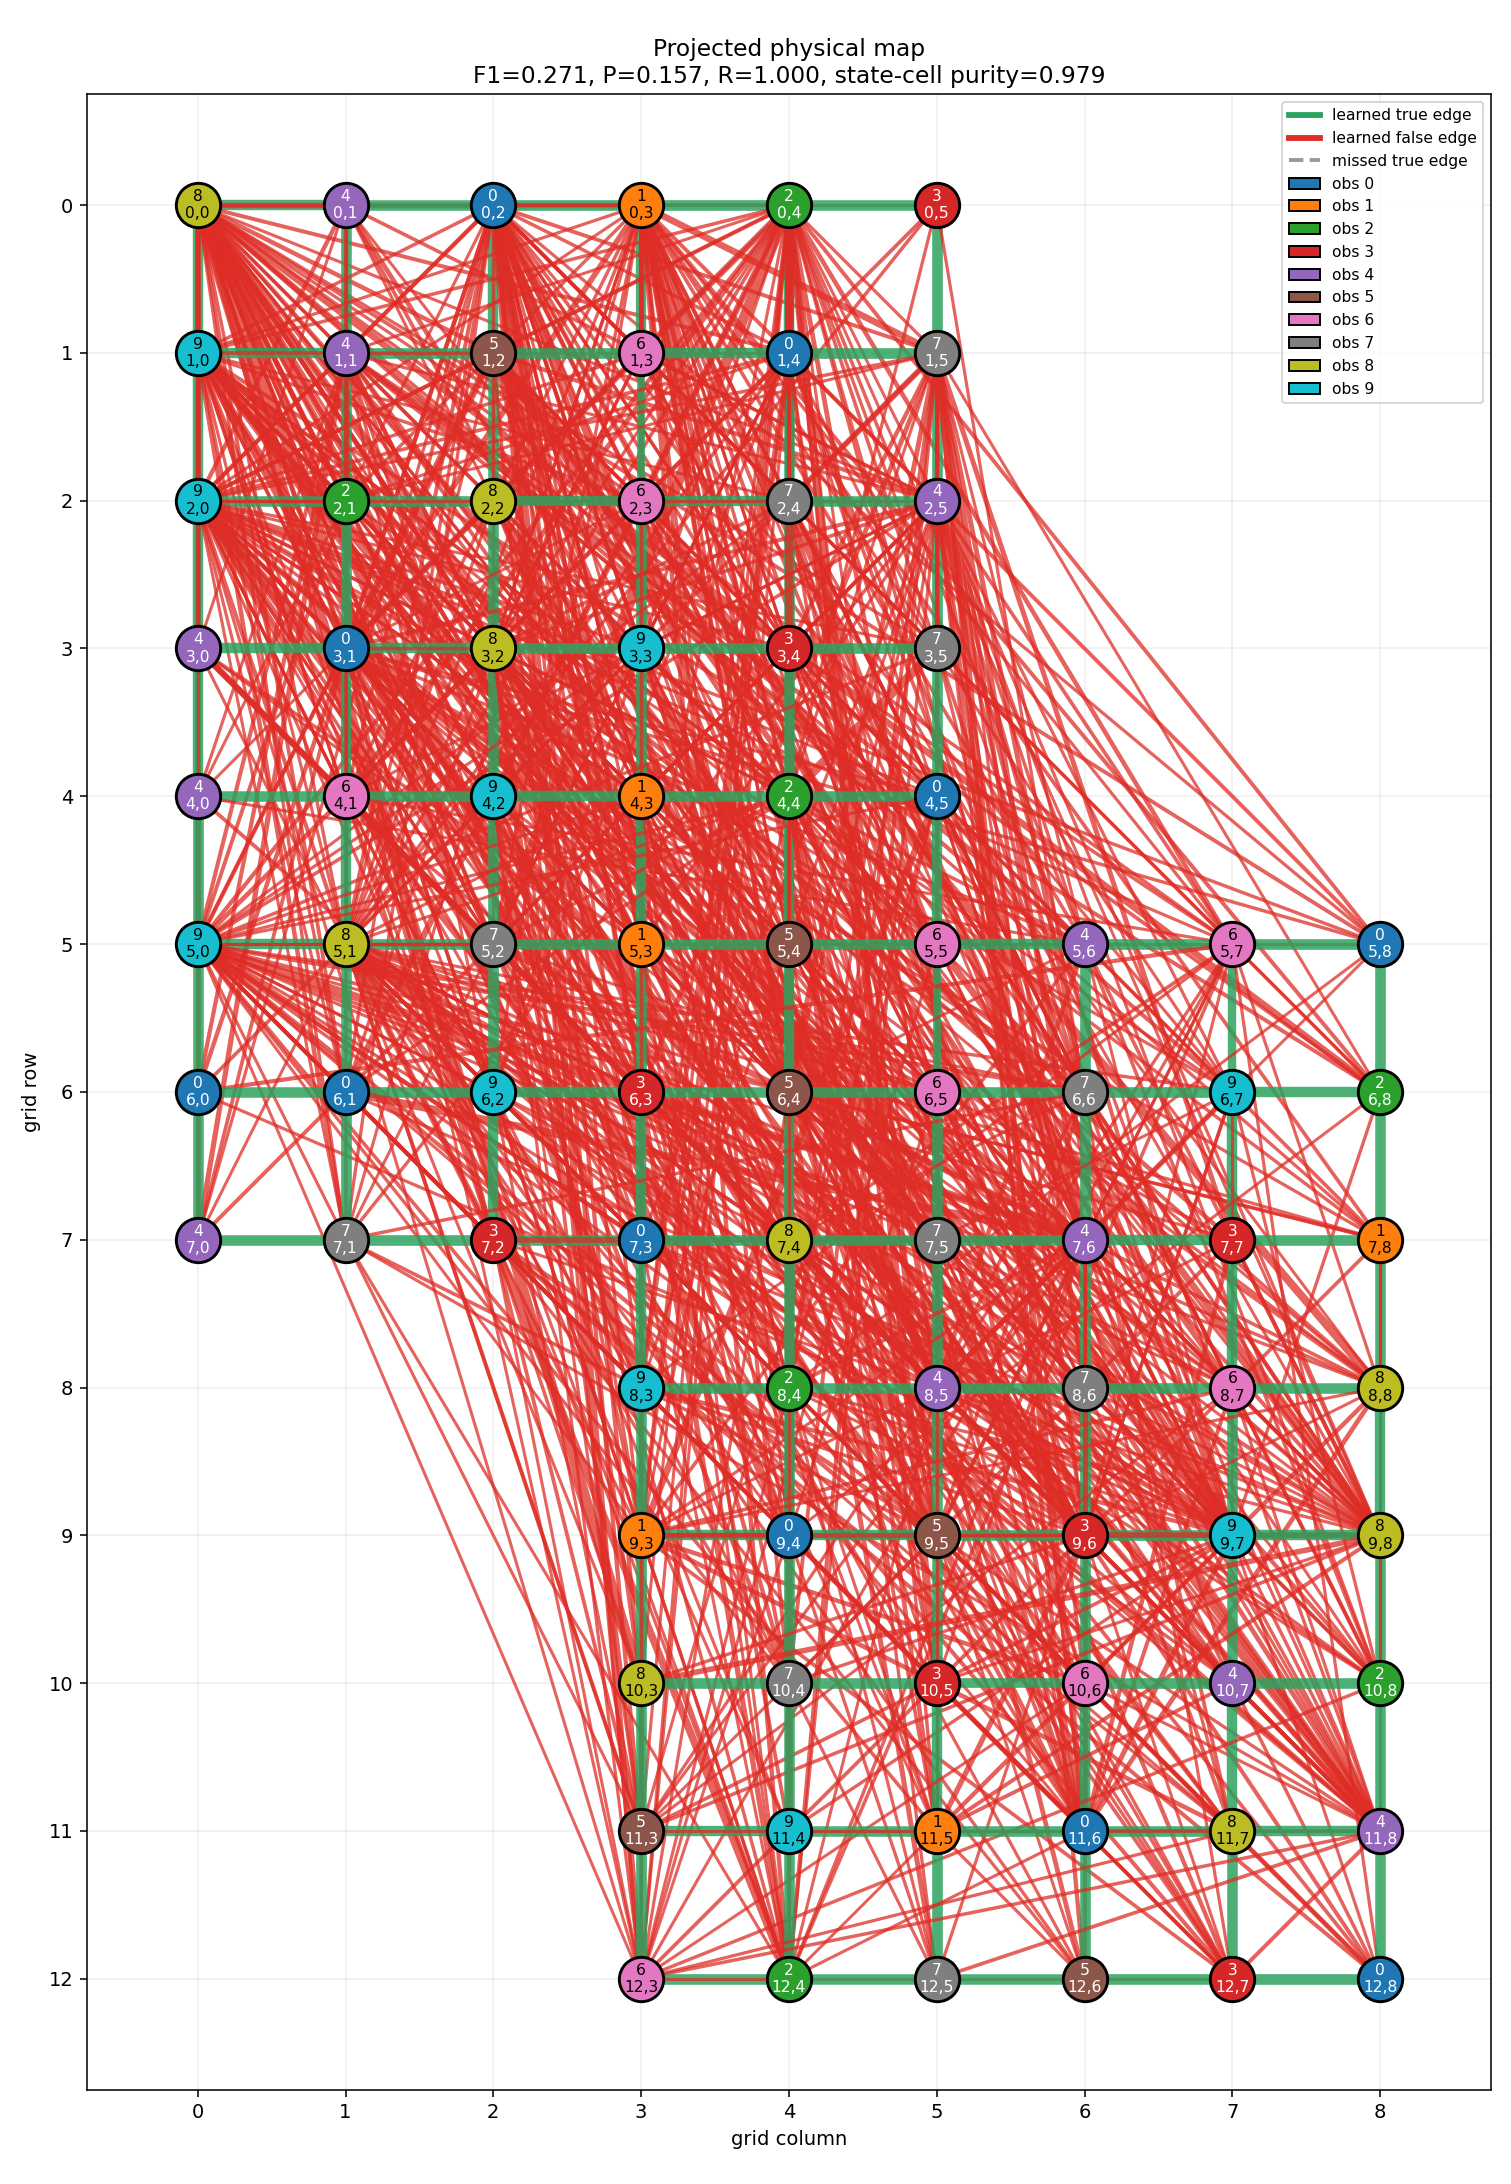
\includegraphics[height=0.62\textheight,keepaspectratio]{projected_physical_graph.png}\\[-0.1em]
      {\scriptsize\color{mutedgray}\texttt{two\_rooms} learned map projected on the true grid.
       \textcolor{goodgreen}{Green}: correct edges. \textcolor{badred}{Red}: false. Grey dashed: missed (none).}
    \end{column}
    \begin{column}{0.52\textwidth}
      \begin{itemize}\small\setlength\itemsep{0.25em}
        \item \textbf{Map-edge recall $= 1.00$ in every scored run.}
        \item The learned graph \emph{contains} the entire true map.
        \item Precision rises sharply with the edge threshold.
      \end{itemize}
      \vspace{0.3em}
      \centering\scriptsize
      \begin{tabular}{@{}ccccc@{}}
        \toprule
        $\eta$ & $0.01$ & $0.05$ & $0.10$ & $0.30$\\
        \midrule
        Precision & $0.24$ & $0.29$ & $0.39$ & $\mathbf{0.77}$\\
        Recall    & $1.00$ & $1.00$ & $1.00$ & $1.00$\\
        F1        & $0.39$ & $0.45$ & $0.56$ & $\mathbf{0.87}$\\
        \bottomrule
      \end{tabular}\\[0.15em]
      {\scriptsize\color{mutedgray}Edge-threshold sweep on \texttt{corridors}.}
    \end{column}
  \end{columns}
\end{frame}

\begin{frame}{Results IV --- cross-environment summary}
  \centering
  \scriptsize
  \begin{tabular}{@{}lccccccccc@{}}
    \toprule
    \textbf{Environment} & \textbf{Grid} & \textbf{$K$} & \textbf{$N$} &
    \textbf{Perplexity} & \textbf{Clone pur.} &
    \textbf{State$\to$place} & \textbf{Action acc.} &
    \textbf{Map recall} & \textbf{Best F1}\\
    \midrule
    \texttt{aliased}        & $4\times4$  & $4$  & $21$  & $4.00$ & $0.84$ & --- & --- & --- & ---\\
    \texttt{corridors}      & $5\times5$  & $6$  & $31$  & $5.71$ & $0.86$ & $0.98$ & $\mathbf{1.00}$ & $1.00$ & $\mathbf{0.87}$\\
    \texttt{room} (uniform) & $6\times6$  & $10$ & $201$ & $6.63$ & $\mathbf{0.90}$ & $0.98$ & $0.94$ & $1.00$ & $0.67$\\
    \texttt{room} (dynamic) & $6\times6$  & $10$ & $57$  & $6.56$ & $0.83$ & $0.95$ & $0.97$ & $1.00$ & $0.85$\\
    \texttt{two\_rooms}     & $13\times9$ & $10$ & $151$ & $9.46$ & $0.88$ & $0.98$ & $0.99$ & $1.00$ & $0.86$\\
    \bottomrule
  \end{tabular}

  \vspace{0.9em}
  \begin{columns}[T,onlytextwidth]
    \begin{column}{0.5\textwidth}
      \begin{block}{Headline}
        \textbf{100\% map-edge recall} on every environment with the metric
        suite; clone-state purity \textbf{0.95--0.98}; action-outcome accuracy
        \textbf{0.94--1.00}.
      \end{block}
    \end{column}
    \begin{column}{0.5\textwidth}
      \begin{itemize}\small\setlength\itemsep{0.15em}
        \item Scales smoothly from $4{\times}4$ to $13{\times}9$.
        \item Dynamic clones get most of the F1 with $4\times$ fewer states.
        \item Open frontier: \textbf{precision} at small thresholds.
      \end{itemize}
    \end{column}
  \end{columns}
\end{frame}

\begin{frame}{Training dynamics --- the phases work as intended}
  \centering
  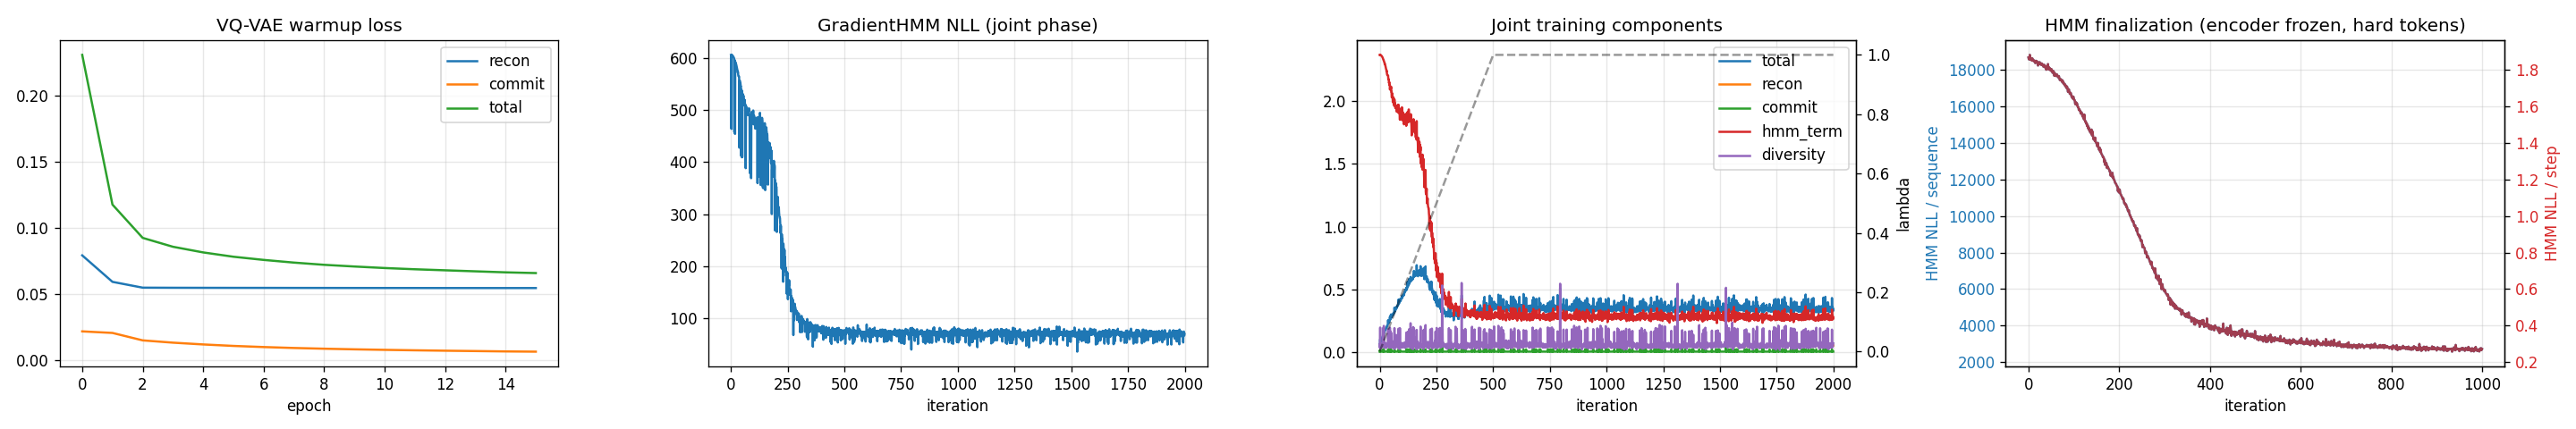
\includegraphics[width=0.93\linewidth]{loss_curves.png}\\
  \vspace{0.3em}
  {\footnotesize\color{mutedgray}\texttt{two\_rooms}: VQ-VAE warmup,
  joint-phase components (reconstruction, commitment, length-normalized HMM,
  diversity), and the pure-HMM finalization.}

  \vspace{0.6em}
  \begin{itemize}\small\setlength\itemsep{0.2em}
    \item Reconstruction stays \textbf{stable} through joint training $\Rightarrow$ no collapse.
    \item Length-normalized HMM term \textbf{decreases steadily} once
          $\lambda_t$ ramps in.
    \item Finalization (encoder frozen) drives a final sharp drop in HMM NLL.
  \end{itemize}
\end{frame}

% =====================================================================
\section{Limitations \& Outlook}
% =====================================================================

\begin{frame}{What still doesn't work as well as it should}
  \begin{columns}[T,onlytextwidth]
    \begin{column}{0.5\textwidth}
      \textbf{Perception bottleneck}
      \begin{itemize}\small\setlength\itemsep{0.15em}
        \item Each observation collapses to \emph{one} integer token.
        \item Severely limits how much an agent can ``see''.
        \item Codebook size is a hard scalability cap.
        \item \textbf{Dynamic clone allocation} helps but is still primitive.
      \end{itemize}

      \vspace{0.4em}
      \textbf{Edge precision}
      \begin{itemize}\small\setlength\itemsep{0.15em}
        \item Recall is perfect; precision is threshold-dependent.
        \item Many \emph{weak} false edges remain in the learned graph.
        \item Needs sharper transition regularization.
      \end{itemize}
    \end{column}
    \begin{column}{0.5\textwidth}
      \textbf{Scaling and training cost}
      \begin{itemize}\small\setlength\itemsep{0.15em}
        \item Forward recursion is sequential in time $\Rightarrow$ slow.
        \item Transition tensor is $O(A \cdot N^2)$ in memory.
        \item Joint training is delicate; every knob matters.
        \item Learning is slower than it should be.
      \end{itemize}

      \vspace{0.4em}
      \textbf{Scope}
      \begin{itemize}\small\setlength\itemsep{0.15em}
        \item Validated on controlled MNIST gridworlds.
        \item Not yet a 3-D image-based environment.
      \end{itemize}
    \end{column}
  \end{columns}
\end{frame}

\begin{frame}{Maybe another way --- RNN-CSCG and exponential RNNs}
  \begin{columns}[T,onlytextwidth]
    \begin{column}{0.55\textwidth}
      \begin{itemize}\setlength\itemsep{0.4em}
        \item Replace the cloned HMM with a \textbf{recurrent neural network}
              constrained to preserve cloning semantics.
        \item Hidden state $h_t$ evolves as
        \[
          h_{t+1} = f_\theta(h_t, a_t, \rho_{t+1}),
        \]
        with $f_\theta$ chosen to keep transitions sparse and orthogonal.
        \item \textbf{Exponential / orthogonal RNNs} could realize the
              "orthogonalized state machine" highlighted by the hippocampal
              study --- the very property that linked CSCGs to the brain in
              the first place.
      \end{itemize}
    \end{column}
    \begin{column}{0.43\textwidth}
      \centering
      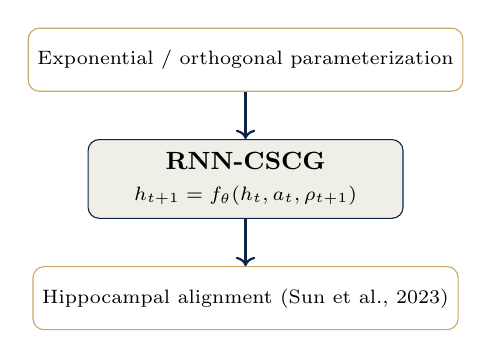
\begin{tikzpicture}[font=\small]
        \node[draw=deepblue,fill=softgray,rounded corners,
              minimum width=4cm,minimum height=1cm,align=center] (rnn)
              {\textbf{RNN-CSCG}\\\scriptsize $h_{t+1}=f_\theta(h_t,a_t,\rho_{t+1})$};
        \node[draw=accentgold,rounded corners,minimum width=4cm,
              minimum height=0.8cm,align=center,above=0.6cm of rnn]
              (exp) {\scriptsize Exponential / orthogonal parameterization};
        \node[draw=accentgold,rounded corners,minimum width=4cm,
              minimum height=0.8cm,align=center,below=0.6cm of rnn]
              (br)  {\scriptsize Hippocampal alignment (Sun et al., 2023)};
        \draw[->,deepblue,thick] (exp) -- (rnn);
        \draw[->,deepblue,thick] (rnn) -- (br);
      \end{tikzpicture}
    \end{column}
  \end{columns}
  \vspace{0.4em}
  \begin{center}\itshape\color{deepblue}
    Same inductive bias, more scalable substrate.
  \end{center}
\end{frame}

\begin{frame}{Take-aways}
  \begin{enumerate}\setlength\itemsep{0.3em}\small
    \item CSCGs carry a useful, neuroscientifically anchored inductive bias for
          cognitive maps --- but classical EM training isolates them from modern
          deep learning.
    \item A \textbf{log-space, differentiable forward pass} turns the CSCG
          into a first-class neural module (\textbf{gradCSCG}).
    \item Coupling gradCSCG to a \textbf{VQ-VAE} via a soft codebook posterior
          gives the first end-to-end pipeline from \emph{pixels to cognitive map}.
    \item Joint training is made stable by principled loss balancing
          (length normalization, $\lambda$-annealing, diversity penalty).
    \item On MNIST gridworlds we recover topology with \textbf{100\%
          edge recall} and \textbf{state-to-place purity 0.95--0.98}.
    \item The frontier: \emph{richer perception}, \emph{sharper transitions},
          and a \textbf{scalable RNN-CSCG} successor.
  \end{enumerate}
\end{frame}

\begin{frame}[plain,noframenumbering]
  \begin{tikzpicture}[remember picture,overlay]
    \fill[deepblue] (current page.south west) rectangle (current page.north east);
    \node[anchor=center] at (current page.center) {%
      \begin{minipage}{0.8\paperwidth}
        \centering
        {\color{accentgold}\rule{2em}{2pt}}\\[1.0em]
        {\color{white}\fontsize{40}{44}\selectfont\bfseries Thank you.}\\[0.8em]
        {\color{white!85}\fontsize{14}{16}\selectfont\itshape Questions \& discussion welcome.}\\[1.2em]
        {\color{accentgold}\rule{2em}{2pt}}\\[1.5em]
        {\color{white!75}\small Arash Nikzad \quad$\cdot$\quad Supervisor: Dr.~Tristan Stober}\\[0.3em]
        {\color{white!60}\scriptsize\texttt{neuralCSCG} \;\textbar\; preprint and code in the project repository}
      \end{minipage}
    };
  \end{tikzpicture}
\end{frame}

\end{document}
